\documentclass[tikz]{standalone}
\usepackage{cancel}
\usepackage{fontspec}
\setmonofont[]{Ubuntu Mono}

\begin{document}
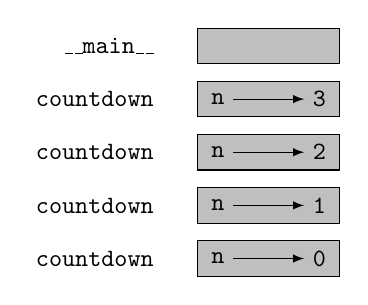
\begin{tikzpicture}[scale=0.9, transform shape]
$\node[anchor=east] at(-1.5,0){\tt \_\_main\_\_};
\node[draw, fill=lightgray, minimum width=2cm, minimum height=0.5cm]{};
\node[anchor=east] at(-1.5,-0.75){\tt countdown};
\node[draw, fill=lightgray, minimum width=2cm, minimum height=0.5cm] at(0,-0.75){};
\node[anchor=east] (n1) at(-0.5, -0.75) {\tt n};
\node[anchor=west] (n1v) at (0.5, -0.75) {\tt 3};
\draw[-latex] (n1) -- (n1v);
\node[anchor=east] at(-1.5,-1.5){\tt countdown};
\node[draw, fill=lightgray, minimum width=2cm, minimum height=0.5cm] at(0,-1.5){};
\node[anchor=east] (n2) at(-0.5, -1.5) {\tt n};
\node[anchor=west] (n2v) at (0.5, -1.5) {\tt 2};
\draw[-latex] (n2) -- (n2v);
\node[anchor=east] at(-1.5,-2.25){\tt countdown};
\node[draw, fill=lightgray, minimum width=2cm, minimum height=0.5cm] at(0,-2.25){};
\node[anchor=east] (n3) at(-0.5, -2.25) {\tt n};
\node[anchor=west] (n3v) at (0.5, -2.25) {\tt 1};
\draw[-latex] (n3) -- (n3v);
\node[anchor=east] at(-1.5,-3){\tt countdown};
\node[draw, fill=lightgray, minimum width=2cm, minimum height=0.5cm] at(0,-3){};
\node[anchor=east] (n4) at(-0.5, -3) {\tt n};
\node[anchor=west] (n4v) at (0.5, -3) {\tt 0};
\draw[-latex] (n4) -- (n4v);
$
\end{tikzpicture}
\end{document}
